\documentclass[tikz]{standalone}

\usepackage{amsmath}

\usetikzlibrary{arrows,positioning}

\begin{document}
	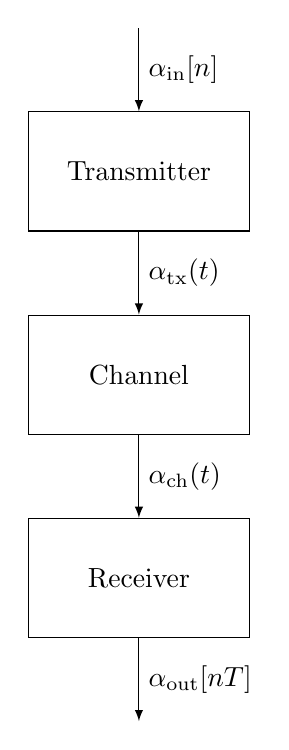
\begin{tikzpicture}[
		node distance=3em,
		arrow/.style={-latex},
		block/.style={draw, minimum height=10ex, minimum width=8em, align=center},
	]
		\coordinate (in) at (0,0);
		\node (tx) [block, below=of in] {Transmitter};
		\node (ch) [block, below=of tx] {Channel};
		\node (rx) [block, below=of ch] {Receiver};
		\coordinate[below=of rx] (out);
		
		\draw[arrow] (in) -- node[anchor=west]{$\alpha_\text{in}[n]$} (tx);
		\draw[arrow] (tx) -- node[anchor=west]{$\alpha_\text{tx}(t)$} (ch);
		\draw[arrow] (ch) -- node[anchor=west]{$\alpha_\text{ch}(t)$} (rx);
		\draw[arrow] (rx) -- node[anchor=west]{$\alpha_\text{out}[nT]$} (out);
	\end{tikzpicture}
\end{document}